\usepackage{tikz}
\usepackage{xstring}

% Aquí van todas las figuras en TikZ, hay que asignarlas un numero para poder cambiar todas a la vez.

\newcommand{\figura}[1]{
	\IfEqCase{#1}{
		{1}{\figurahipA}
		{2}{\figurahipB}
		{3}{\pizarra}
		{4}{\figurahipBfin}
	}[\PackageError{figura}{Figura no declarada: #1}{}]
}


% Aqui se añaden las figuras %
\newcommand{\figurahipA}{
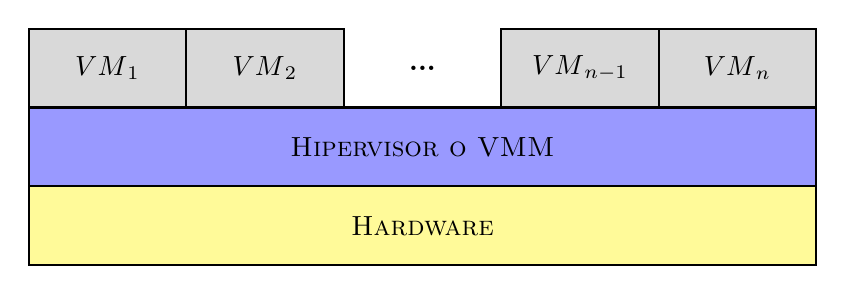
\begin{tikzpicture}
	\draw[fill=gray!30, thick] (0,2) rectangle (2,3);
	\draw[fill=gray!30, thick] (2,2) rectangle (4,3);
	\draw[fill=gray!30, thick] (6,2) rectangle (8,3);
	\draw[fill=gray!30, thick] (8,2) rectangle (10,3);
	\draw[fill={blue!40}, thick] (0,1) rectangle (10,2); 
	\draw[fill=yellow!40, thick] (0,0) rectangle (10,1); 

	\node at (1,2.5) {${VM}_1$};
	\node at (3,2.5) {${VM}_2$};
	\node at (5,2.5) {\textbf{...}};
	\node at (7,2.5) {${VM}_{n-1}$};
	\node at (9,2.5) {${VM}_n$};
	\node at (5,1.5) {\textsc{Hipervisor o VMM}};
	\node at (5,0.5) {\textsc{Hardware}};
\end{tikzpicture}
}

\newcommand{\figurahipB}{
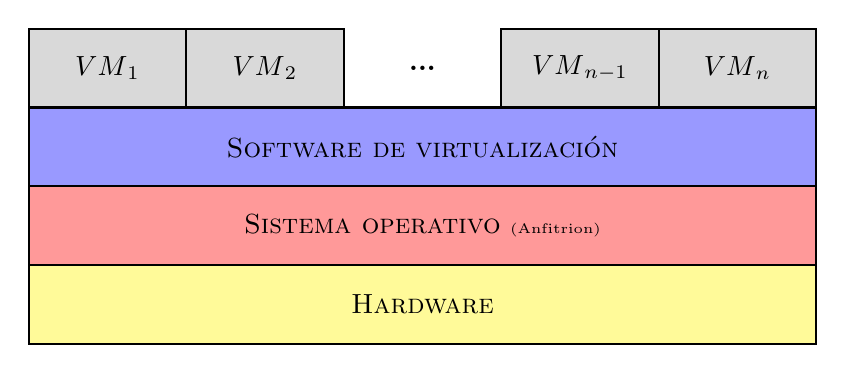
\begin{tikzpicture}
	\draw[fill=gray!30, thick] (0,3) rectangle (2,4);
	\draw[fill=gray!30, thick] (2,3) rectangle (4,4);
	\draw[fill=gray!30, thick] (6,3) rectangle (8,4);
	\draw[fill=gray!30, thick] (8,3) rectangle (10,4);
	\draw[fill={blue!40}, thick] (0,2) rectangle (10,3);
	\draw[fill={red!40}, thick] (0,1) rectangle (10,2); 
	\draw[fill=yellow!40, thick] (0,0) rectangle (10,1); 

	\node at (1,3.5) {${VM}_1$};
	\node at (3,3.5) {${VM}_2$};
	\node at (5,3.5) {\textbf{...}};
	\node at (7,3.5) {${VM}_{n-1}$};
	\node at (9,3.5) {${VM}_n$};
	\node at (5,2.5) {\textsc{Software de virtualización}};
	\node at (5,1.5) {\textsc{Sistema operativo} {\tiny (Anfitrion)}};
	\node at (5,0.5) {\textsc{Hardware}};
\end{tikzpicture}
}

\newcommand{\figurahipBfin}{
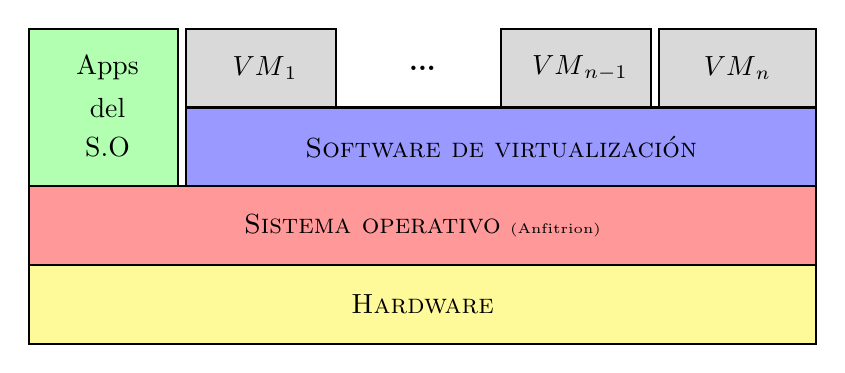
\begin{tikzpicture}
	\draw[fill=green!30, thick] (0,2) rectangle (1.9,4);
	\draw[fill=gray!30, thick] (2,3) rectangle (3.9,4);
	\draw[fill=gray!30, thick] (6,3) rectangle (7.9,4);
	\draw[fill=gray!30, thick] (8,3) rectangle (10,4);
	\draw[fill={blue!40}, thick] (2,2) rectangle (10,3);
	\draw[fill={red!40}, thick] (0,1) rectangle (10,2); 
	\draw[fill=yellow!40, thick] (0,0) rectangle (10,1); 

	\node at (1,3.5) {Apps};
	\node at (1,3) {del};
	\node at (1,2.5) {S.O};
	\node at (3,3.5) {${VM}_1$};
	\node at (5,3.5) {\textbf{...}};
	\node at (7,3.5) {${VM}_{n-1}$};
	\node at (9,3.5) {${VM}_n$};
	\node at (6,2.5) {\textsc{Software de virtualización}};
	\node at (5,1.5) {\textsc{Sistema operativo} {\tiny (Anfitrion)}};
	\node at (5,0.5) {\textsc{Hardware}};
\end{tikzpicture}
}

\newcommand{\pizarra}{
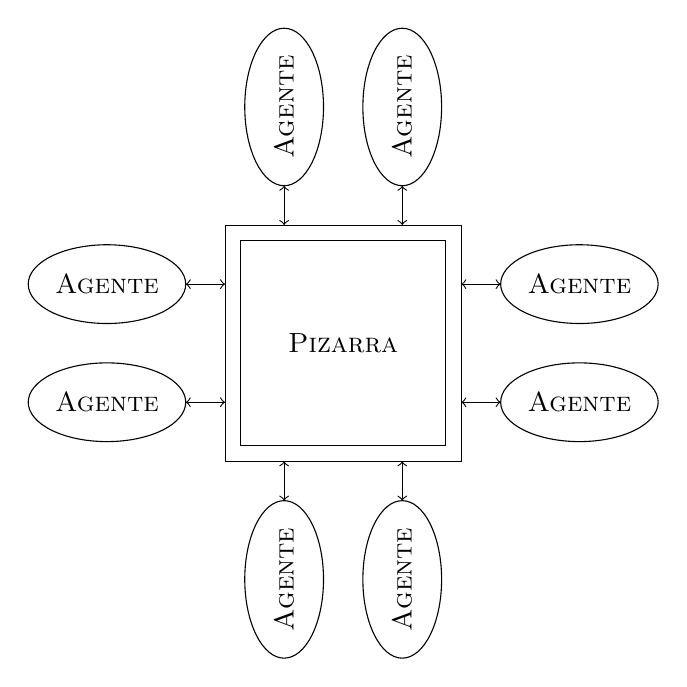
\begin{tikzpicture}
	\draw (0,0) rectangle (3,3);
	\draw (0.2, 0.2) rectangle (2.8,2.8);
	\draw (4.5,2.25) ellipse (1cm and 0.5cm);
	\draw (4.5,0.75) ellipse (1cm and 0.5cm);
	\draw (0.75,-1.5) ellipse (0.5cm and 1cm);
	\draw (2.25,-1.5) ellipse (0.5cm and 1cm);
	\draw (-1.5,0.75) ellipse (1cm and 0.5cm);
	\draw (-1.5,2.25) ellipse (1cm and 0.5cm);
	\draw (0.75,4.5) ellipse (0.5cm and 1cm);
	\draw (2.25,4.5) ellipse (0.5cm and 1cm);
	
	\draw[<->] (3,0.75) -- (3.5,0.75);
	\draw[<->] (3,2.25) -- (3.5,2.25);
	\draw[<->] (0.75,3) -- (0.75,3.5);
	\draw[<->] (2.25,3) -- (2.25,3.5);
	\draw[<->] (0,0.75) -- (-0.5,0.75);
	\draw[<->] (0,2.25) -- (-0.5,2.25);
	\draw[<->] (0.75,-0.5) -- (0.75,0);
	\draw[<->] (2.25,-0.5) -- (2.25,0);
	
	\node at (1.5,1.5) {\textsc{Pizarra}};
	\node at (4.5,2.25) {\textsc{Agente}};
	\node at (4.5,0.75) {\textsc{Agente}};
	\node[rotate=90] at (0.75,-1.5) {\textsc{Agente}};
	\node[rotate=90] at (2.25,-1.5) {\textsc{Agente}};
	\node at (-1.5,0.75) {\textsc{Agente}};
	\node at (-1.5,2.25) {\textsc{Agente}};
	\node[rotate=90] at (0.75,4.5) {\textsc{Agente}};
	\node[rotate=90] at (2.25,4.5) {\textsc{Agente}};
\end{tikzpicture}
}
